\section{Binary--mixture periodic in 3-dimensions}
The existence of a temperature gradient in the system should not be able to generate a net flow in the fluid. 
This point is discussed by Levich who describes how the flow at the interface should be accompanied by a back-flow in the bulk fluid.\cite{Levich}
In the case of the binary--mixture held between two walls, the walls are held stationary and provide a momentum sink which allows a net flow to exist within the fluid.
To replicate the behaviour described by Levich one must study a system with no such momentum sinks, for example a simple periodic system of two immiscible fluids as shown on the left--hand side of Figure \ref{SetUp}.

This system was prepared from a FCC lattice of Lennard--Jones particles and the parameters described in Section \ref{InteractionModel} and using a Nos\'e--Hoover thermostat and barostat.
To create the fluid state, the systems were equilibrated for $2 \times 10^{6}$ timesteps (of length $\delta t = 0.001\ \tau$) at a pressure of $P^{*} = 0.1$ and temperatures of $T^{*}=0.8$ and $T^{*}=0.9$.

\subsection{Comparing the Virial and Irving--Kirkwood stress}
Once again there is an ambiguity over which stress--tensor should be used for calculating the fluid stress profile.
Initially, both $\sigma^{\mathrm{V}}$ and $\sigma^{\mathrm{IK}}$ were computed for the symmetric--binary mixture.
This was achieved by running the equilibrated systems for $10 \times 10^{6}$ timesteps over which period the number--density, $\sigma^{\mathrm{V}}$ and $\sigma^{\mathrm{IK}}$ were calculated for 400 spatial bins.
As discussed before, the Irving--Kirkwood analysis was very computationally expensive and this simulation length was the upper feasible limit.
\FloatBarrier

\begin{figure}[h]
\centering
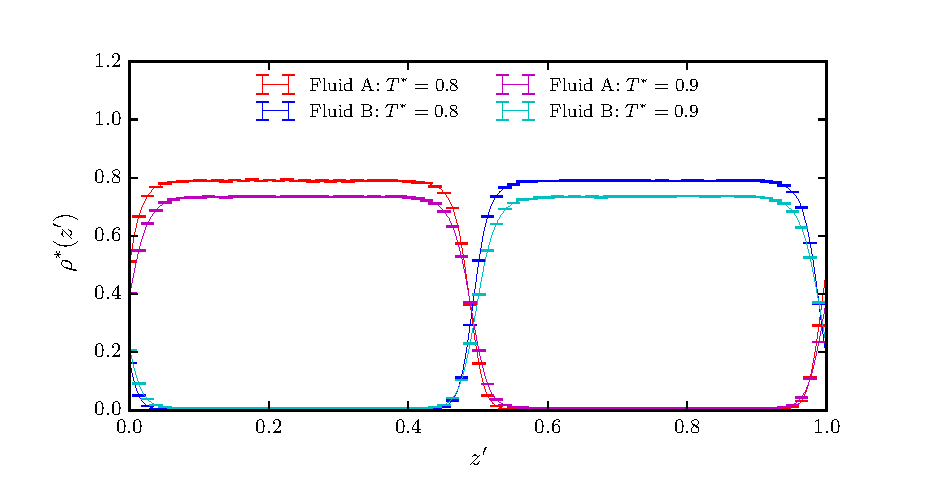
\includegraphics[scale=0.8]{Period10Rho}
\caption{Period10Rho}
\label{Period10Rho}
\end{figure}
After this period the density profile (plotted in Figure \ref{Period10Rho}) clearly showed a uniform fluid density in the fluid bulk and a sharp interfacial region as expected.
However, it is clear that the exact position of the interface had shifted slightly during the simulation and was no longer coincedent for the two temperatures.
This would have severe consequences when calculating the Marangoni force from the stress profile and thus this shift had to be manually corrected by recentering the interfaces prior to computing the finite difference
\FloatBarrier

\begin{figure}[h]
\centering
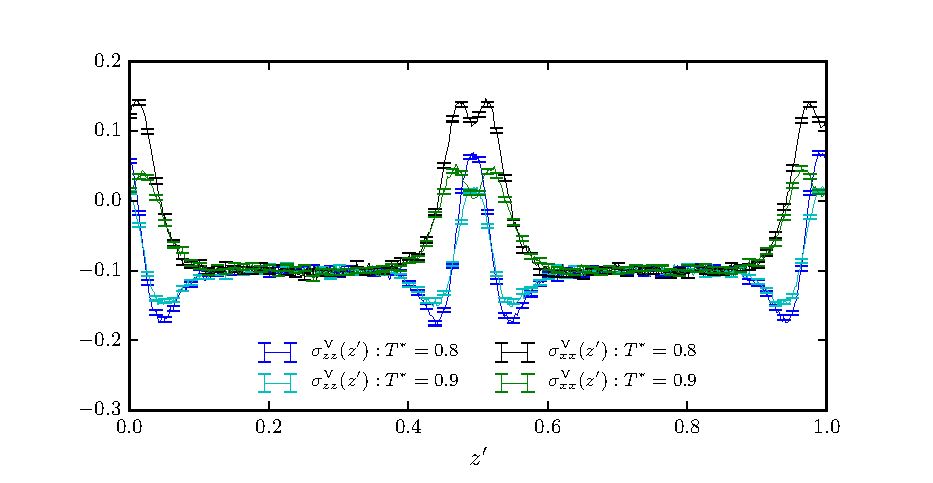
\includegraphics[scale=0.8]{Period10VirStress}
\caption{Period10VirStress}
\label{Period10VirStress}
\end{figure}

\begin{figure}[h]
\centering
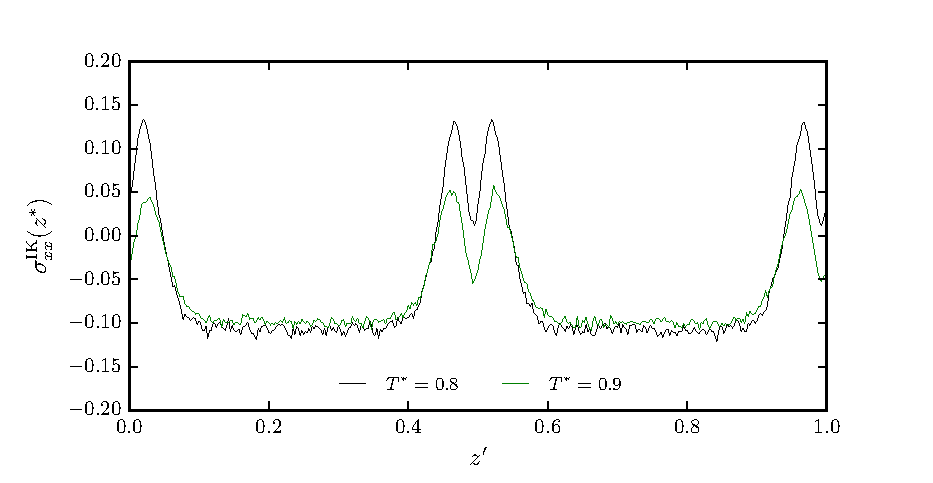
\includegraphics[scale=0.8]{Period10IKStress}
\caption{Period10IKStress}
\label{Period10IKStress}
\end{figure}
The recentered Virial and Irving--Kirkwood stress profiles are plotted in Figure \ref{Period10VirStress} and Figure \ref{Period10IKStress} respectively.
As with the fluid confined between two walls, the stress--tensor components are equal to $-P_{\mathrm{ext}}$ in the bulk of the fluid correpsonding to the hydrostatic fluid pressure.
There is a peak in both the Virial and Irving--Kirkwood stress at the interface, again as a result of the anistropy of the interparticle forces in this region.
These peaks have the same maximum value for both stress--tensors although the Irving--Kirkwood stress shows a stronger minimum directly at the interface.

\FloatBarrier
Using these force profiles the gradient of the stress with repsect to temperature was calculated from the finite difference approach.
For there to be no net force acting on the fluid there must be some source of momentum sink in the system, for example a distant wall bounding the fluid.
No such momentum sink exists for the infinite fluid represented by this system, therefore the force profile must be adjusted to give no net force.
To achieve this the average force was subtracted from the force profile fixing ensuring that the integral of the force profile over all space was zero as shown in Figure \ref{Period10Force}.

\begin{figure}[h]
\centering
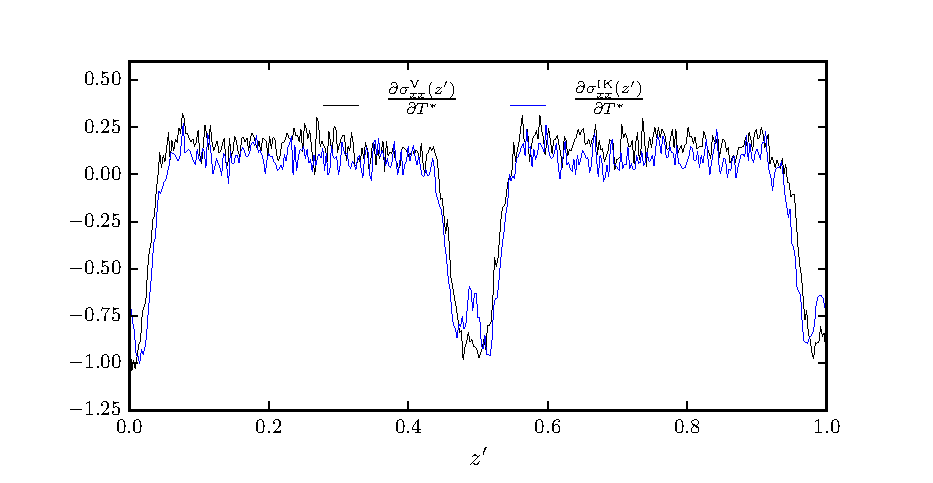
\includegraphics[scale=0.8]{Period10Force}
\caption{Period10Force}
\label{Period10Force}
\end{figure}
The resulting force profile shows a similar peak at the interface to seen in Figure \ref{PisIKForce} with a similar maximum value suggesting that fixing the total force on the fluid to zero correctly adjusts the data to give a physically meaningful Marangoni force.
Again there is a reasonably good correspondence between the force calculated using the Irving--Kirkwood and Virial stress--tensors although directly at the interface the magnitude of the peak is reduced for the Irving--Kirkwood force.
Away from the interface there is a bulk force acting in the opposite direction to the interfacial Marangoni force that will generate the expected bulk backflow.
However the profile as a whole shows too much noise for the fine--structure of the force to be determined and thus is not of a sufficient quality to be used as an artificial body--force in a non--equilibrium simulation.

\subsection{Reducing the noise in the force--profile}
To generate a force profile with a sufficiently low level of nosie that it can be used as an artifical body force in a non-equilibrium run requires either a larger system size or a longer simulation timescale.
Both of these increase the computational cost of calculating the Irving--Kirkwood stress--tensor beyond a practical level and thus to achieve a more accurate force profile, the Virial stress--tensor must be used.
Considering how similar the Virial and Irving--Kirkwood force profiles appear in Figure \ref{PisIKForce}, using the Virial stress--tensor to calculate the Marangoni force will not create too much deviation from the force that could be calculated from the more suitable Irving--Kirkwood stress--tensor whilst it would enable a much longer simulation time to achieved practically.
\FloatBarrier

\begin{figure}[h]
\centering
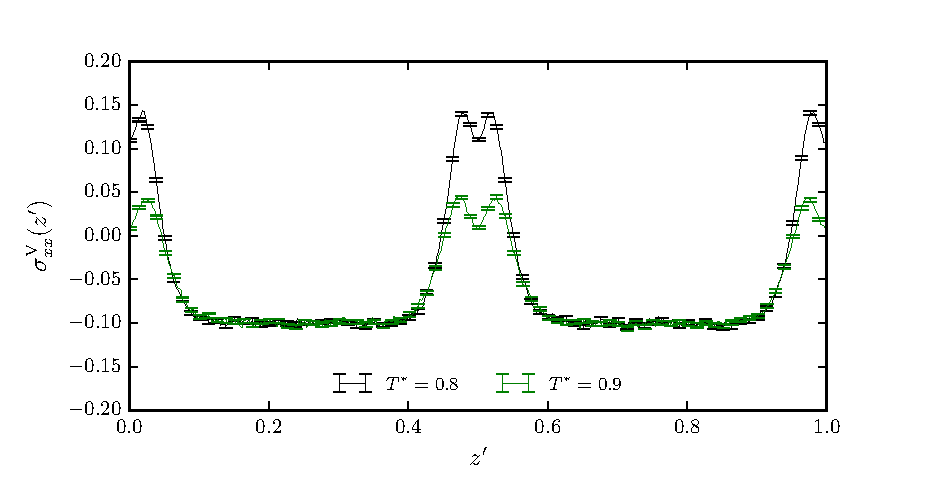
\includegraphics[scale=0.8]{Period30VirStress}
\caption{Period30VirStress}
\label{Period30VirStress}
\end{figure}

The reduced noise stress--profile was generated by running the equilibrium systems at $T^{*}=0.8$ and $T^{*}=0.9$ for $30 \times 10^{6}$ timesteps and spatially averaging the Virial stress--tensor every timestep.
These values were then time--averaged (again using a block length of $10,000$) and the interfaces were recentered to generate the stress profile shown in Figure \ref{Period30VirStress}.
For both temperatures the stress--profile shows much less noise, especially in the bulk region, for the longer simulation run and the interfacial peaks in the tangential stress--tensor is more symmetric.
\FloatBarrier

\begin{figure}[h]
\centering
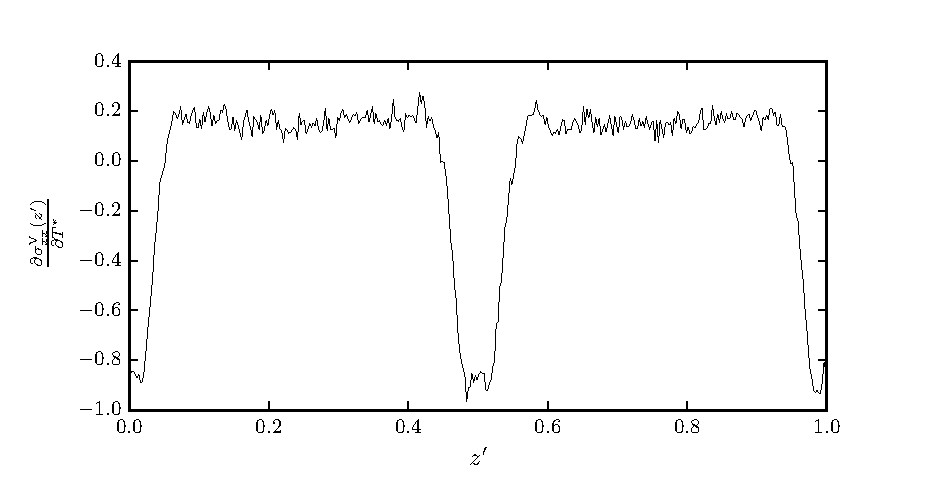
\includegraphics[scale=0.8]{Period30VirForce}
\caption{Period30VirForce}
\label{Period30VirForce}
\end{figure}
Using this stress profile the gradient of the stress--tensor with respect to temperaturee may again be computed using the finite difference and then the average value may be subtracted to give the profile shown in Figure \ref{Period30VirForce}.
There is a dramatic reduction in the noise of this force profile compared to Figure \ref{Period10Force} and the profile clearly shows a sharp peak at the interface and a back force in the bulk regions.
\FloatBarrier

Using the profile given in Figure \ref{Period30VirForce} and a temperature gradient of $\partial T / \partial x^{*} = 0.001$ an artifical body force was computed.
This body force profile was recentered to ensure that the peak corresponding to the Marangoni force aligned with the interfacial region at $T^{*} = 0.85$ and this was applied to a non--equilibrium simulation.
The non--equilibrium simulation was run for $40 \times 10^{6}$ and the x--component of the velocity was outputted every timestep for $400$ spatial bins across the z--dimension. 
These values for the velocity were then time--averaged using the same block length described earlier to yield the velocity profile plotted in Figure \ref{Period30VirFlow}.

\begin{figure}[h]
\centering
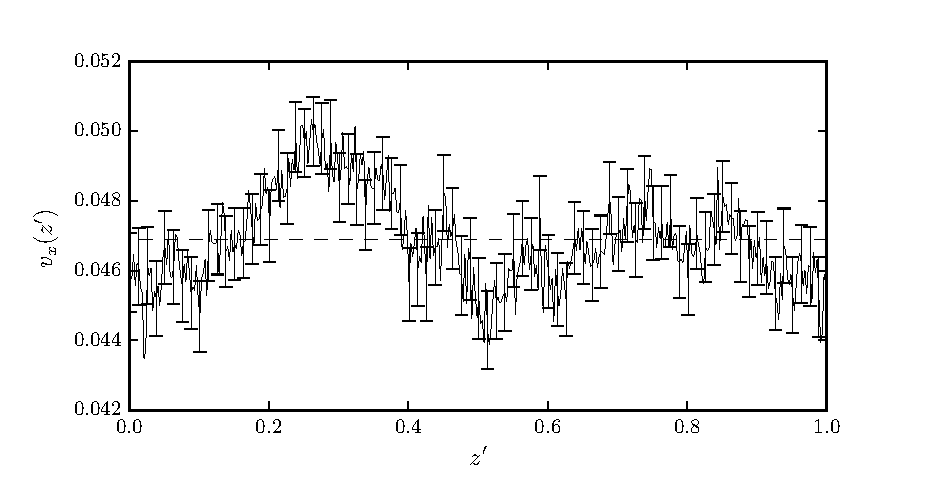
\includegraphics[scale=0.8]{Period30VirFlow}
\caption{Period30VirFlow}
\label{Period30VirFlow}
\end{figure}

This flow profile still retains a lot of statistical noise despite the simulation being run for a long timescale, something which would be difficult to improve upon.
Moreover the average fluid velocity (indicated the hashed line) is non--zero, implying that there is motion of the centre--of--mass during the non-equilibrium run.
This centre--of--mass motion is occuring even though the force--profile has been recentered to give no net force acting on the fluid. 
It is likely that in the absence of a momentum sink in a system like this, it would be very difficult to remove this net fluid flow without fixing the centre--of--mass artificially throughout the simulation.
Despite this, the relative motion across the fluid can still be considered and the form of this does, to some extent, show a velocity peak at the interface (with $v < v_{\mathrm{COM}}$) corresponding to the Marangoni flow and some evidence for the expected back flow in the bulk fluid (with $v > v_{\mathrm{COM}}$).
This result is, however, very ambiguous and there was insufficient time in the project to improve this non--equilibrium simulation.

\subsection{Summary}
Using the binary--mixture periodic in three--dimensions allowed the Marangoni effect to be studied without the influence of external wall effects.
By measuring the stress--tensor at $T^{*}=0.8$ and $T^{*}=0.9$ and calculating the finite difference, the force profile in the fluid resulting from a temperature gradient was computed and this showed a peak at the interface of the two fluids.
It was important to ensure that the interfaces in the two equilibrium simulations were aligned before calculating the finite difference to create a faithful force profile.
Furthermore, as this system has no sources of momentum the force profile had to be adjusted to ensure there was no net force acting on the fluid.

This force was calculated using both the Irving--Kirkwood and Virial stress--tensor, however due to the high computational cost of the Irving--Kirkwood method the simulation could not be run for long enough to reduce the noise sufficiently.
Regardless, both of the methods yielded phenomenologically similar force profiles and thus by computing the Virial stress over a much longer timescale, a more precised force profile could be calcuated.
Using this force--profile in a non-equilibrium simulation produced a net fluid flow, probably an error due to the lack of a momentum sink, but the relative motion of the fluid showed the expected peak at the interface with an opposing back flow in the fluid bulk.


\subsubsection{SUMMARY piston}
The finite difference approach for the fluid confined between two walls showed the Marangoni force could be calculated using the Virial stress--tensor and the Irving--Kirkwood stress--tensor.
Both of these methods produced a similar force at the interface of the two fluids although the Irving--Kirkwood stress--tensor gave a reduction in the force calculate directly at the interface.
By applying these force profiles as an applied body force in a non--equilibrium, the Marangoni flow profile was computed and showed a Couette flow.
The flow profile for the Irving--Kirkwood and Virial stress--tensors was very similar although the Irving--Kirkwood profile was not symmetrical, probably due to increased noise in the Irving--Kirkwood force profile.

\subsubsection{SUMMARY periodic}
Using the binary--mixture periodic in three--dimensions allowed the Marangoni effect to be studied without the influence of external wall effects.
By measuring the stress--tensor at $T^{*}=0.8$ and $T^{*}=0.9$ and calculating the finite difference, the force profile in the fluid resulting from a temperature gradient was computed and this showed a peak at the interface of the two fluids.
It was important to ensure that the interfaces in the two equilibrium simulations were aligned before calculating the finite difference to create a faithful force profile.
Furthermore, as this system has no sources of momentum the force profile had to be adjusted to ensure there was no net force acting on the fluid.

This force was calculated using both the Irving--Kirkwood and Virial stress--tensor, however due to the high computational cost of the Irving--Kirkwood method the simulation could not be run for long enough to reduce the noise sufficiently.
Regardless, both of the methods yielded phenomenologically similar force profiles and thus by computing the Virial stress over a much longer timescale, a more precised force profile could be calcuated.
Using this force--profile in a non-equilibrium simulation produced a net fluid flow, probably an error due to the lack of a momentum sink, but the relative motion of the fluid showed the expected peak at the interface with an opposing back flow in the fluid bulk.
